%
% Based on File acl2017.tex
%
%% Based on the style files for ACL-2015, with some improvements
%%  taken from the NAACL-2016 style
%% Based on the style files for ACL-2014, which were, in turn,
%% based on ACL-2013, ACL-2012, ACL-2011, ACL-2010, ACL-IJCNLP-2009,
%% EACL-2009, IJCNLP-2008...
%% Based on the style files for EACL 2006 by 
%%e.agirre@ehu.es or Sergi.Balari@uab.es
%% and that of ACL 08 by Joakim Nivre and Noah Smith

\documentclass[11pt,a4paper]{article}
\usepackage[hyperref]{acl2017}
\usepackage{times}
\usepackage{latexsym}
\usepackage{color}
\usepackage[ngerman, english]{babel}
\usepackage[utf8]{inputenc}
\usepackage[pdftex]{graphicx}

\usepackage{url}

\usepackage{booktabs}

% own package declarations
\usepackage{mdwlist}
\usepackage{paralist}
\usepackage{siunitx}
\usepackage{subfigure}
%\usepackage{numprint}\npthousandsep{,}\npthousandthpartsep{}\npdecimalsign{.}

\aclfinalcopy 

\newcommand\BibTeX{B{\sc ib}\TeX}

%change title
\title{Single Token Part-of-Speech Tagging using Support Vector Machines and Word Embedding Features}

%change name and mail
\author{Andreas Funke \\
  {\tt andreas.funke@hhu.de} \\
}
\date{}

\begin{document}
\maketitle
\begin{abstract}
Part-of-speech tagging (POS) is a common technique in Natural Language Processing pipelines. It enriches a corpus with grammatical information which can be exploited not only for syntactic but also for semantic evaluation. In this paper we propose an SVM based POS-tagger trained on the TIGER corpus using word embeddings of small dimensionality as input data. The feature-set is based only on the token itself without context of surrounding words. A maximum F$_1$ micro score of 0.919 when tested on the HDT corpus could be achieved.

\end{abstract}



\section{Introduction}
Part-of-speech tagging (POS) is a common technique in Natural Language Processing pipelines. By annotating each word of a corpus with its word-class, succeeding processes can benefit from these additional features. POS tagging enriches a corpus with grammatical information which can be exploited not only for syntactic but also for semantic evaluation. For example it can be used to solve problems such as word disambiguations and phrase dependencies.

POS-tagging can be based on a dictionary, rule based or based on a machine learning model. The latter requires the tagger to be trained on a (semi-)manually annotated corpus. Since POS-tagging is highly language dependent like most other NLP tasks, the training data should fulfill obvious language requirements. For the German language the TIGER \cite{Brants2004} and HDT \cite{Foth14} corpora are some of the best sources for high quality pre-annotated part-of-speech data.

The challenge for this paper is to define a feature-set for a Support Vector Machine (SVM) based POS-tagger \cite{nakagawa2001unknown}. SVMs are common models for supervised machine learning. They are binary classifiers which during training attempt to find an optimal linear hyperplane discrimination two given classes. For non-linear separable data, SVMs can use a non-linear kernel function to transform the data set into a higher dimensional feature space where the data becomes linearly separable. Combinations of separately trained SVMs can be used multi-class problems.

We will use the TIGER corpus to train an SVM and the HDT corpus for test predictions. The corpora are annotated with the widespread (that is for the German language) STTS \cite{schiller1999} tagset. Both using slightly different dialects. We mapped their default tagsets to a reduced universal tagset, consisting of 12 classes \cite{petrov2011universal}.

Since SVMs accept numerical inputs, but NLP corpora contain words, we propose the use of word embeddings to quantize given string-tokens. Word embeddings are a way to vectorize words in a relatively small vector space. Traditional word vectorization methods rely on one-hot-encoding, i.e. a vector with a 1 on a position corresponding to the position of the word in the vocabulary, and 0 on all other fields \cite{hinton1984distributed}. One-hot-encoding for large vocabularies will result in a vector space with a dimensionality (= size of the vocabulary) and very sparse vectors.

Word embedding on the other hand is a method to project this high dimensionality to a much smaller fixed-sized vector space while also embedding syntactic and semantic meaning into the feature space. Word embeddings can be produced with prediction based (e.g. word2vec \cite{mikolov2013efficient}) or count based (e.g. GloVe \cite{pennington2014glove}) learning mechanisms. They will result in a dense real-valued vector space usually with a selectable dimensionality of 50-500.

Support Vector Machines don't scale well with a high input dimensionality, especially if upscaling kernel functions such as rbf (radial basis function -- required for this challenge) are applied. Therefore, we argue that small sized word embeddings are an efficient and effective way to train an SVM as POS-tagger using only a minimal feature-set -- the token itself.



\section{System Description}
For the challenge we faced a few fixed comparability-constraints: Using the libsvm based scikit-learn \cite{scikit-learn} SVC class with the default rbf-kernel was mandatory. Apart from that, parameters could be tweaked to taste. Especially the input features should be chosen to surpass a baseline F$_1$ measure of 0.65 in the classification score. Beside choosing a feature set, preprocessing of feature values plays another important role. Scikit-learn was used in version 0.17.1, since this is the version currently available on the University's high performance computer (HPC) where training and tests were conducted.


\subsection{Support Vector Machine}
Using the SVC class with default parameters is straightforward, once a feature vector is present. We are challenged with a multi-class problem, while SVMs are by design binary classifiers. We've left the default value for the decision function at one-versus-rest (ovr), which results in $K = 12$ SVMs trained. A one-versus-one (ovo) approach would result in $K(K-1)/2 = 66$ SVMs being trained, which was not applicable.

No class weights were applied, although this could be interesting to evaluate. For deployment on the high performance cluster we've chosen a cache-size of 26GB. The default arguments for the parameters gamma, probability, tolerance and random-state stayed untouched, although in hindsight specifying a seed might have been a good idea for reproducibility. We will elaborate on the other parameters in the evaluation section.

The two-dimensional input matrices for each training and test data have the size $|dataset\;items| \times |features|$. In general, C-ordered numpy arrays or sparse vectors (recommended for one-hot-encodings) can be used. For word-embeddings numpy arrays are mandatory since their vectors are not sparse. The gold-labels for each input token are enum-like integers representing one the 12 available classes from the universal tagset. The TIGER and HDT corpus annotations have been mapped to this tagset in advance using basically the proposed mapping in \cite{univmap}.


\subsection{Features}
Part-of-speech tagging is usually context sensitive, which means the surrounding words of a token contain inherent information about its word class. This can be used for example to solve word disambiguations. The context -- i.e preceding and succeeding two words -- should make a good prediction about a POS-tag, even without looking at the token itself. To solve problems such as handling out of vocabulary tokens, we could also look at character n-grams, especially pre- and suffixes of a token, for example the first and last 4 characters of a word. Word-beginnings (case-sensitivity) as well as -endings are often very common for certain word-categories. We could also enrich our tokens with there lemmata which both corpora kindly provide.

Let's assume we chose the four surrounding four as features, the token itself as well as its first and last 4 character n-grams and additionally the token's lemma. If we use scikit-learn's DictVectorizer class to quantize these features with one-hot-encodings we would end up with a feature-vector in size of about $600000$.

Therefore, we will do none of the above. Instead we will focus on the token itself and not on its context. It is clear, that some problems like word disambiguations can not be solved without context, but apart from that we want to see how well the SVM works as POS-tagger with such a restricted feature-set. Our approach is therefore to exploit the syntactic and semantic clustering of word embeddings.

In a first attempt to reduce out-of-vocabulary issues we have taken one of the biggest per-trained word-vector corpus freely available for the German language, the fastText embeddings. The corpus was trained on German Wikipedia articles. The vectors have a dimensionality of 300  and 6GB in size (plain text). Still, roughly 1/3 of the words in the vocabulary of the HDT and TIGER corpus are not contained in the fastText vocabulary. FastText provides a mechanism to deal with out-of-vocabulary tokens by exploiting n-gram similarities, but we weren't able to experiment with this feature. Our endeavor to use this embedding had to be abandoned after several attempts, as the SVM would not finish training even after 24h training time with plenty of CPU-power and memory resources on the 
University's high performance cluster.

Although a feature-vector of size 300 should still be manageable for a SVM, the dense real-values in word-vectors in combination with the rbf-kernel seem to challenge the optimization beyond the systems resources. Since we couldn't find another adequate corpus with lower dimensionality, we trained our own word-vectors from both the TIGER and HDT corpus. At least for the data of this challenge we would furthermore get rid of out-of-vocabulary issues.

The custom word vectors have been trained using gensim and its Word2Vec model. We trained embeddings for each size in {12, 25, 50, 100}, each with either the CBOW and the skip-gram model and again each of these combinations using lowercase tokens or keeping case sensitivity. We would therefore end up with 16 different embeddings which we all trained and tested on the SVM-tagger. For the training of the word vectors we used the default Word2Vec settings with negative sampling (negative=5), but set min\_count=0, as our corpora are relatively small and well written with little spelling issues and we wanted to retain vectors for all tokens.
The embedding was done on a local machine using four workers in relatively short time -- around 10 minutes for all 16 embeddings combined. For compilation reasons gensim can not be installed on the HPC. Therefore, we converted the models from gensim's proprietary format to plain python dictionaries before using the vectors as inputs to the SVM.

It is clear that beyond the HDT test-case, where custom word vectors are available, this approach could result in out-of-vocabulary issues, but so would one-hot-encoding as well.


\subsection{Preprocessing}
SVMs are sensitive to the scaling of data. Word embeddings are not normalized by default. The variance is however rather small. Values are in the range of $\pm 3$ more or less evenly distributed on all dimensions. Still, we were curious if scaling of the input data would make any difference. The first attempt was to use the scikit-learn's StandardScaler, which removes the mean and set standard-deviation to unit variance for each dimension . This resulted in some values being up- instead of downscaled in some dimensions. This is not necessarily a problem, but unexpected so we decided for the MinMaxScaler, normalizing all dimensions to [0, 1]. Of course, it is important to keep the scaler and process the test-data with the same scaling factors as the training data. Training was done with and without scaling. On prediction the scaler was used only when the training data was also preprocessed with the scaler.


\subsection{Computational requirements}
Training and testing of each model takes a considerable amount of time -- usually a couple of hours, but up to 24 hours at maximum depending on chosen parameters. It is performed on CPUs and neither libsvm nor scikit-learn do parallelize the computation. With a multi-class one-versus-rest approach, parallelization should not be hard to do, but the HPC utilization was only 1 core out of 8 being used. The same applies for a few locally conducted tests. The memory consumption depends only partly on the size of the feature-vector. Tests with fastText vectors and vector size of 300 could break the 30GB job limit, resulting in failed tests, while training with a vector size of 12 might still utilized still around 20GB, which is why the cache-size was chosen in that range.

Training and test times correspond to each other for a given model. For predictions the duration is a little higher on average, but keep in mind that the test corpus is approx. 5.5 times bigger. To uncouple resources for training and test phases, the training program stores the model, a potential scaler and an option-file with parameter settings and training-time information to the file-system. The test program will pick up these files, scale the data if appropriate and store a result-file with scores and test-time information next to the model.



\section{Evaluation}

\subsection{Data set}
Testing was performed on the HDT corpus which is considerably larger than the TIGER corpus. HDT consists of $4853410$ tokens, while TIGER has only $888237$ tokens. So, HDT is around 5.5 times bigger, which is a somewhat unusual for machine learning, where the test corpus is usually significantly smaller than the training corpus.

Both corpora were taken from German media sources and were and semi-automatically annotated. The TIGER Corpus from the university of Stuttgart, currently available in version 2.2, uses articles from the German newspaper Frankfurter Rundschau. The HDT (Hamburg Dependency Treebank, v1.0.1) from the University of Hamburg is created using articles from the German IT-news site heise.de, focusing on computer related topics.


\subsection{Metrics}
From our discouraging experience with large sized word embeddings, one of the first metrics was the training-time and the parameter sensitivity on this key figure. Considering the size of the test corpus, the prediction duration was another interesting metric. It is however noteworthy, that runtime-durations should be taken with a grain of salt. Although all trainings were all performed with the same HPC settings, it is difficult to say, if the cluster really provided the same resources to each job.

That being said, the main metric is naturally an evaluation measure for the model's accuracy. An F$_1$ micro score was used for comparison with the baseline. Scikit-learn also provides the F$_1$ macro and F$_1$ weighted scores, which were all evaluated as well. The evaluation is focusing on finding a sweet-spot between runtime-performance (duration of training and test phases) and accuracy-performance (3 provided F$_1$ scores). The following parameters used for training will be analyzed:

\subsubsection{Embedding parameters}
\begin{itemize*}
	\item \emph{Dimensionality:} custom trained word vectors of size 12, 25, 50 and 100. It is expected that a higher size will boost the F$_1$ measures at the cost of speed.
	\item \emph{Model:} CBOW and Skip-gram. This may or may not make a difference.
	\item \emph{Case sensitivity:} lowercased tokens may be beneficial for words at the beginning of sentences, but it may be also prone to word disambiguations.
\end{itemize*}

\subsubsection{Preprocessing}
\begin{itemize*}
	\item \emph{Scaling:} using the MinMaxScaler on the data prior to training and test should in theory result in better performance, as well time-wise as for precision.
	\item \emph{Training set size:} although the challenge expected to train on the complete TIGER corpus we have additionally trained on roughly 1/2 and 1/8 of the corpus.
\end{itemize*}

\subsubsection{SVM parameters}
\begin{itemize*}
	\item \emph{C:} increases the soft margin. Rumor has is, that extremely high values (C = 1000) can be beneficial for highly dimensional inputs, while C = 1 is the default.
	\item \emph{Max\_iter:} this parameter limits the number of iterations within the solver. Limiting this value can greatly speedup the training, potentially at the cost of accuracy. Default is None. Also trained with a value of 1000.
	\item \emph{Shrinking:} libsvm suggested that turning off the shrinking heuristic might speed up the training, considering the given data. So all training were performed without this heuristic.
\end{itemize*}

\subsubsection{Parameter combinations}
\begin{itemize*}
	\item 4 embedding sizes (12, 25, 50, 100)
	\item 2 embedding models (CBOW, Skip-gram)
	\item 2 case settings (lowercase, case-sensitive)
	\item 2 values for C (1.0, 1000.0)
	\item 2 values for max\_iter (None, 1000)
	\item 2 scaling options (with, without)
	\item 2 training set sizes (400k, 888k)
\end{itemize*}

All combined resulting in 256 SVM models trained -- thanks to the HPC. As of yet, not all all models finished testing. Especially models with embedding size of 100 and training set size of 888k took significantly longer as well for training as for testing. Some additional trainings and tests were conducted with a training set size of 100k, for example with C=2.0.

Test results were plotted for each parameter on a time-versus-score plane, distinguishing also for the different training set sizes. Maximum score values, minimum training times and mean values for each parameter were also analyzed.


\subsection{Results}

\begin{figure}[htbp]
	\centering
	\subfigure[Results for parameter max-iter\label{fig:max_iter}]  {\centering
		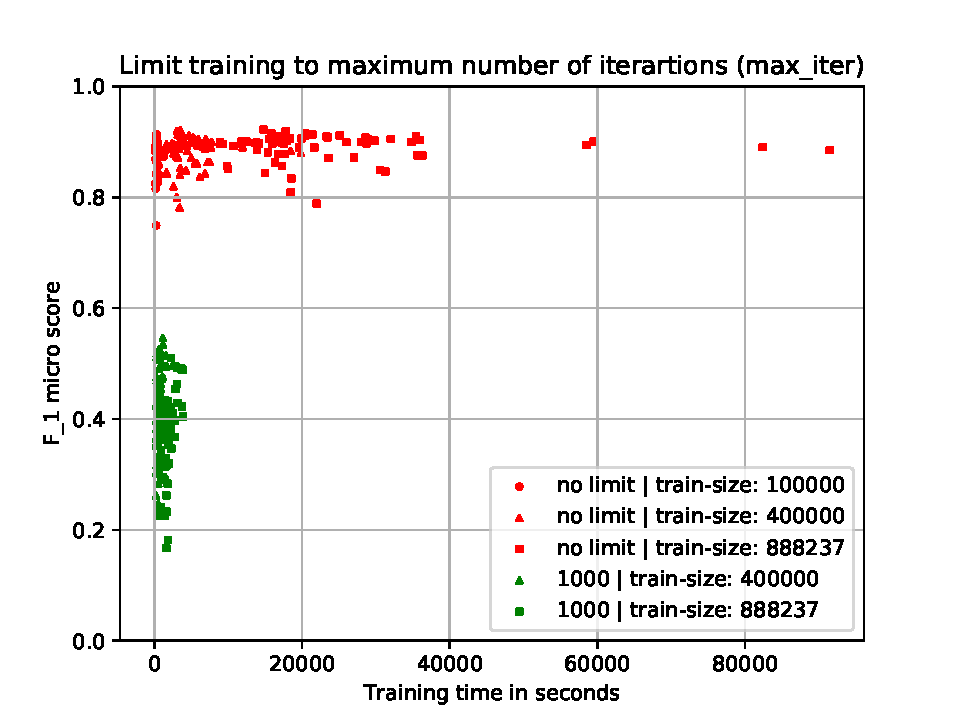
\includegraphics[width=.525\textwidth]{fig/max_iter_train_size__train_time__f1_micro}
	}
	\subfigure[Results for embedding size\label{fig:embedding_size}]  {\centering
		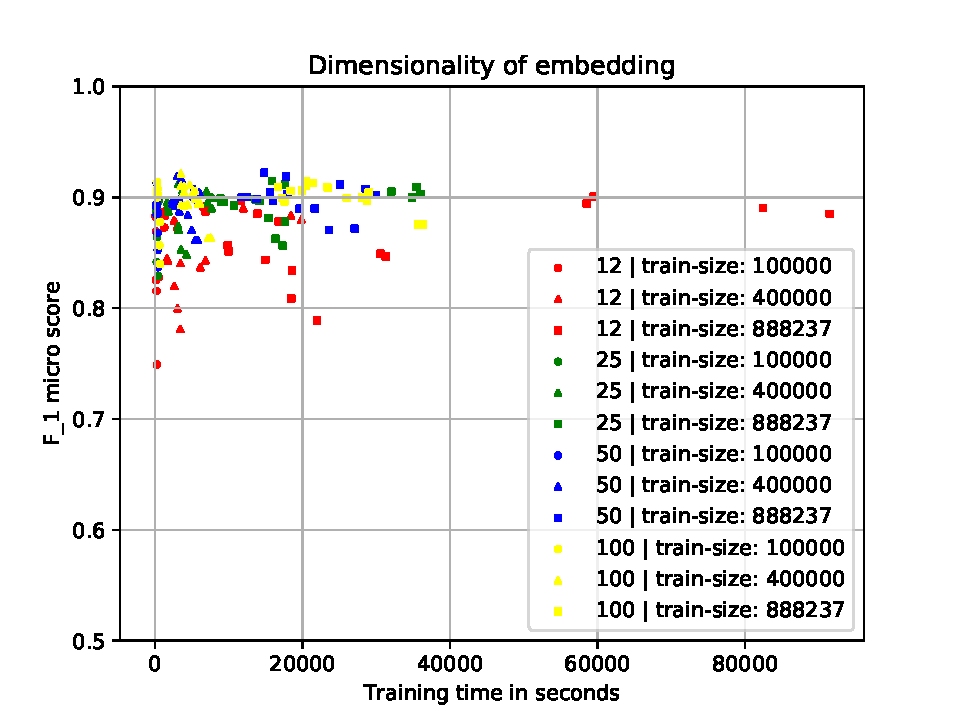
\includegraphics[width=.525\textwidth]{fig/embedding_size_train_size__train_time__f1_micro}
	}
	\subfigure[Results for embedding model\label{fig:embedding_model}]  {\centering
		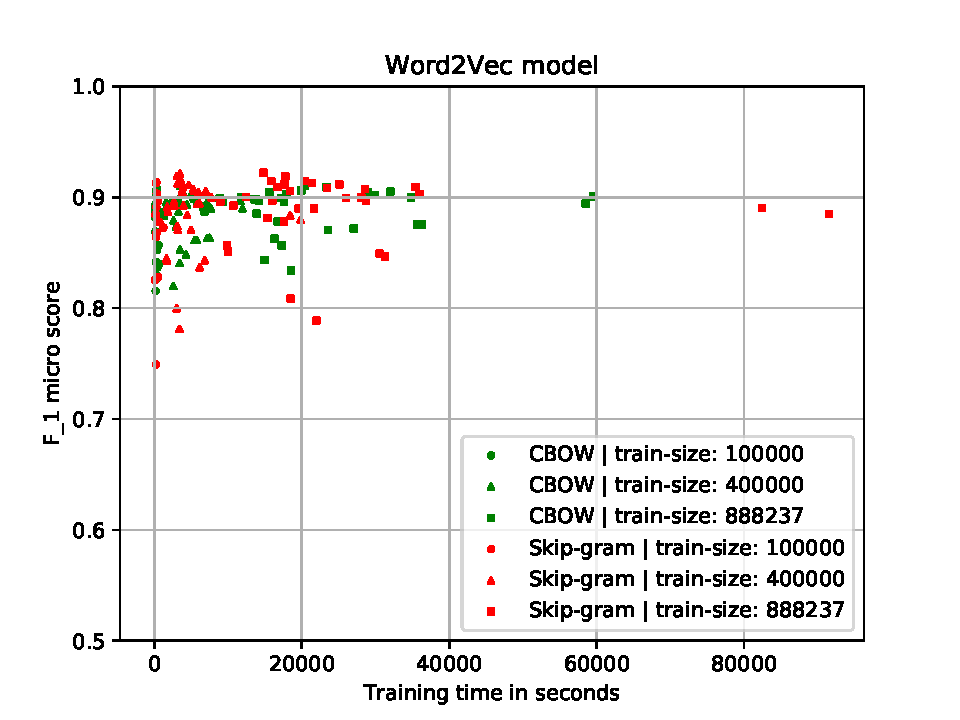
\includegraphics[width=.525\textwidth]{fig/embedding_model_train_size__train_time__f1_micro}
	}
	\caption{Evaluation results per parameter}
	\label{fig:results1}
\end{figure}


\begin{figure}[htbp]
	\centering
	\subfigure[Results for case sensitivity\label{fig:lowercase}]  {\centering
		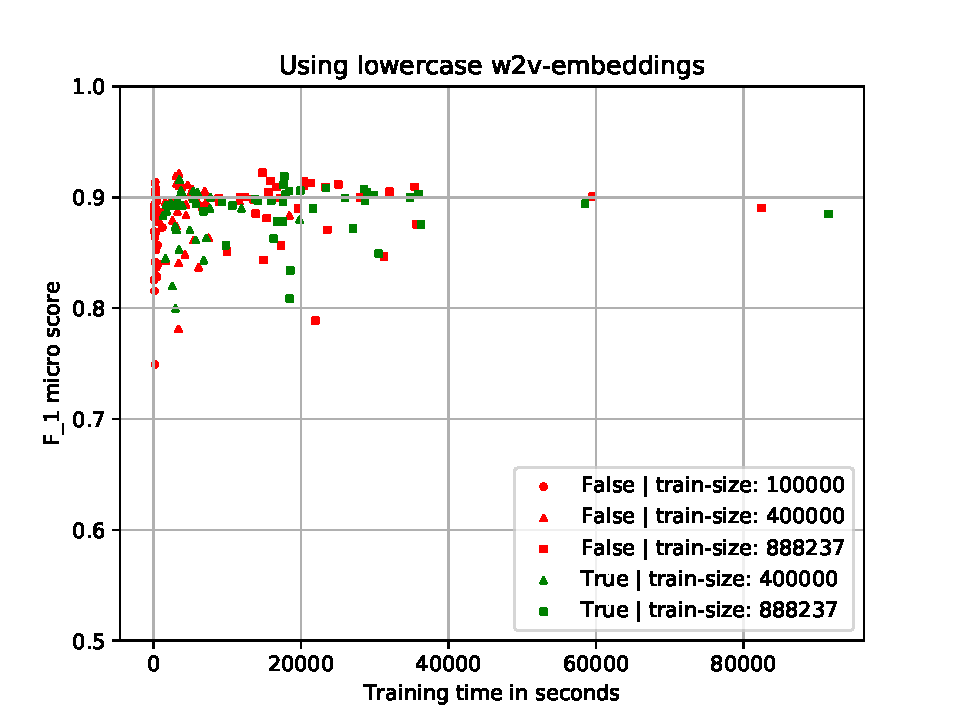
\includegraphics[width=.525\textwidth]{fig/lowercase_train_size__train_time__f1_micro}
	}
	\subfigure[Results for parameter C\label{fig:C}]  {\centering
		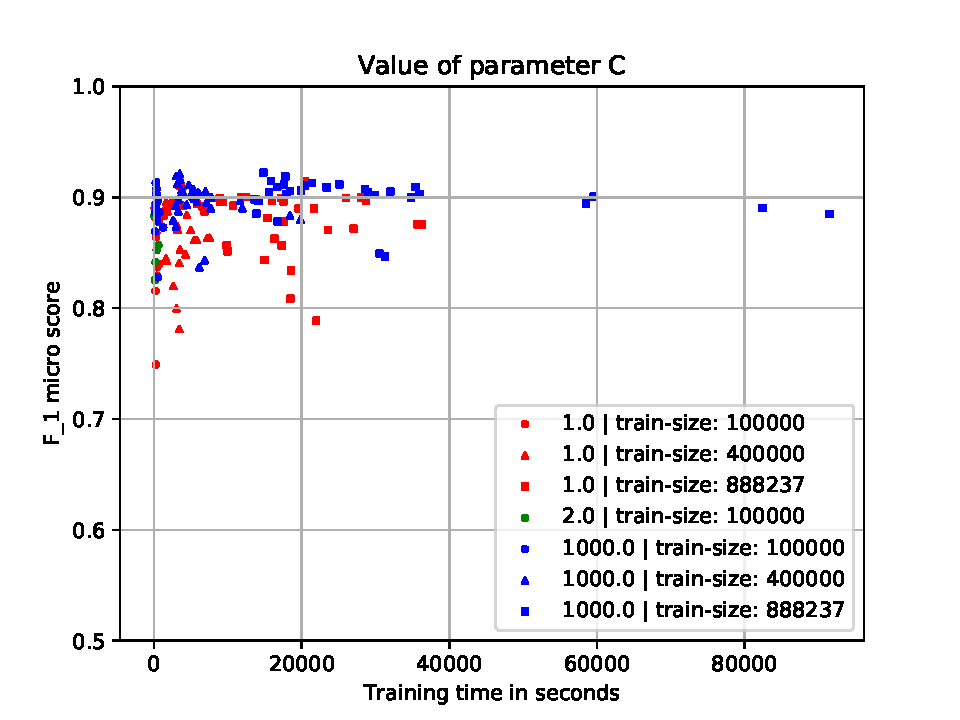
\includegraphics[width=.525\textwidth]{fig/C_train_size__train_time__f1_micro}
	}
	\subfigure[Results for scaling\label{fig:scale}]  {\centering
		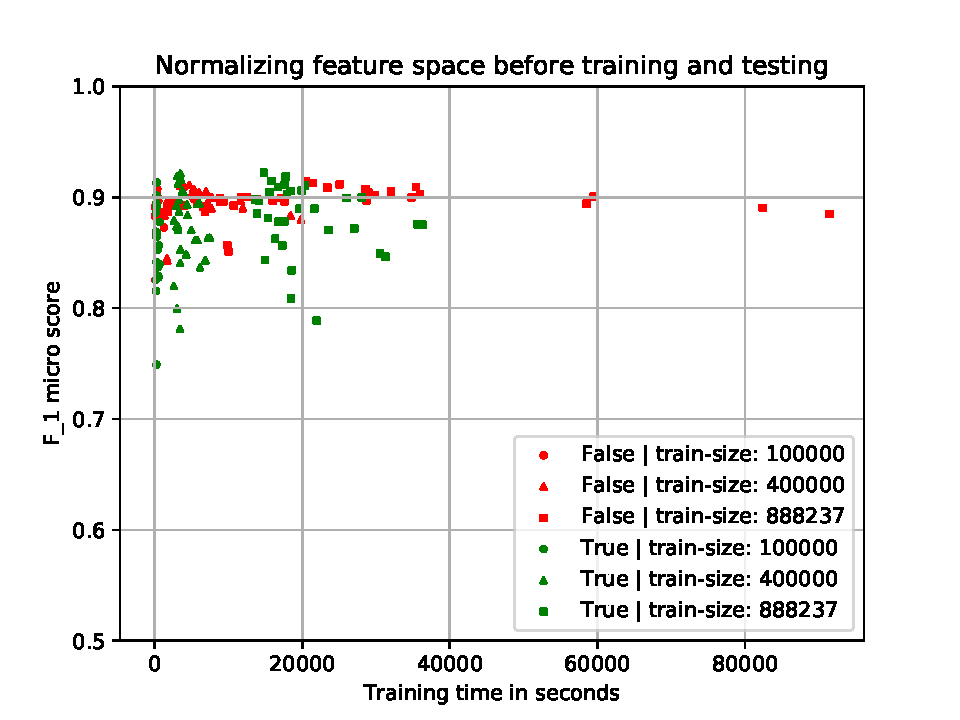
\includegraphics[width=.525\textwidth]{fig/scale_train_size__train_time__f1_micro}
	}
	\caption{Evaluation results per parameter}
	\label{fig:results2}
\end{figure}


\begin{figure}[htbp]
	\centering
	\subfigure[Results for training set size\label{fig:train_size}]  {\centering
		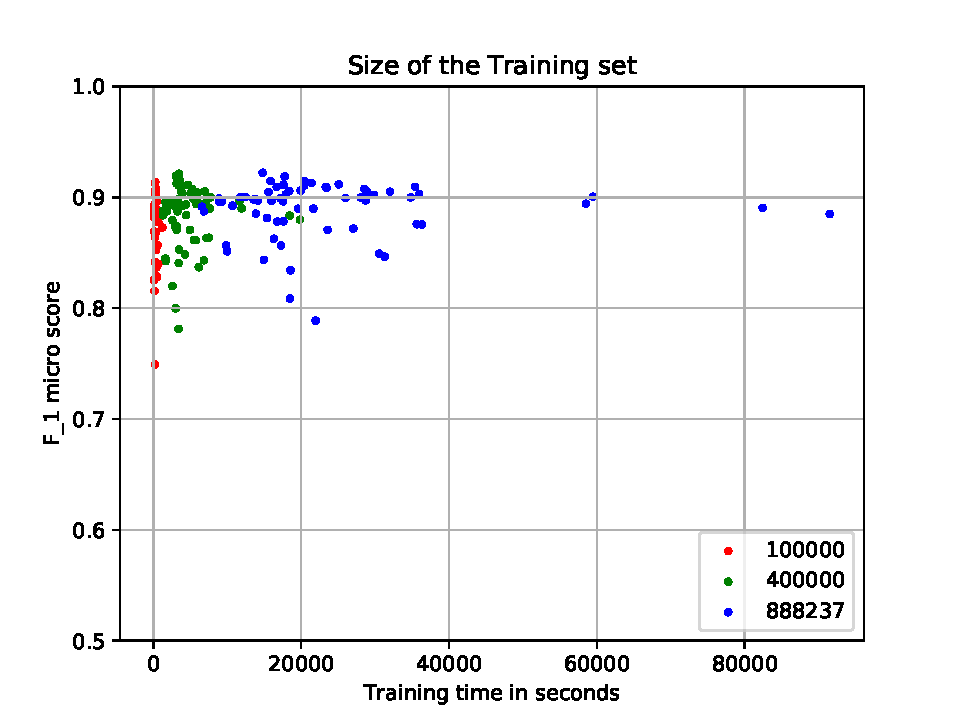
\includegraphics[width=.525\textwidth]{fig/train_size__train_time__f1_micro}
	}
	\subfigure[Results for training set size -- test times\label{fig:train_size_test}]  {\centering
		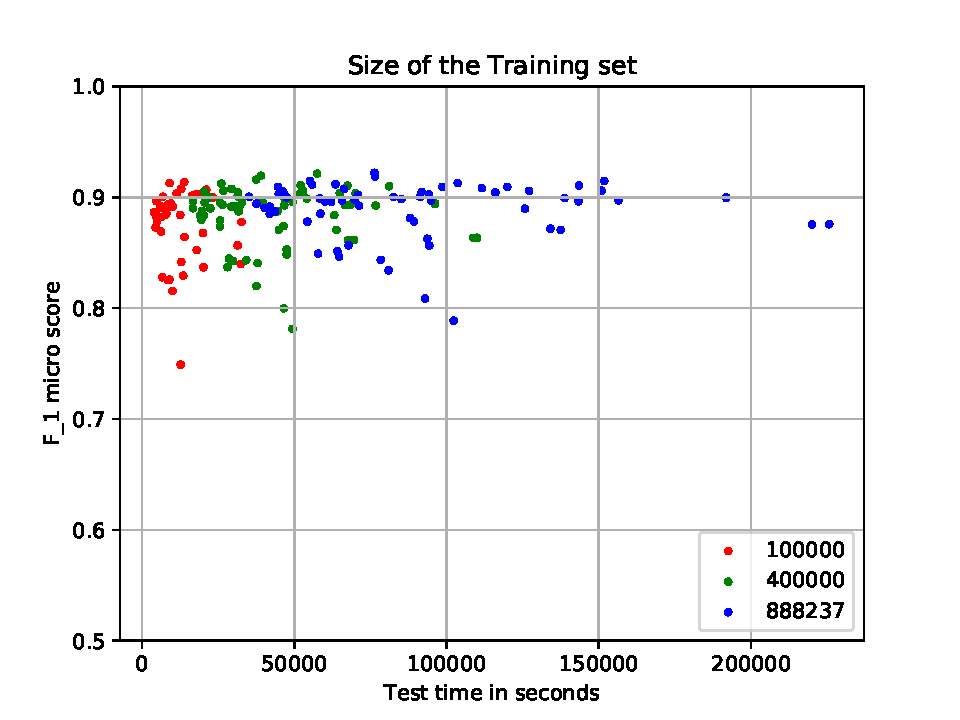
\includegraphics[width=.525\textwidth]{fig/train_size__test_time__f1_micro}
	}
	\caption{Evaluation results per parameter}
	\label{fig:results3}
\end{figure}


%\begin{figure}[htbp]
%	\centering
%	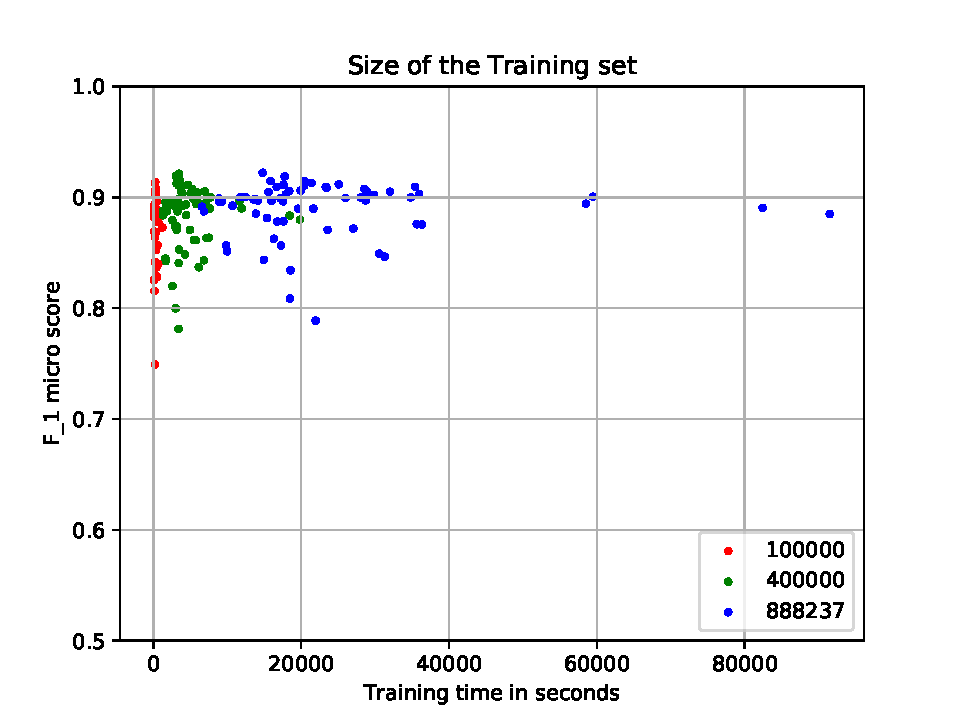
\includegraphics[width=1\linewidth]{fig/train_size__train_time__f1_micro}
%	\caption{Results for training set size}
%	\label{fig:train_size}
%\end{figure}
%
%
%\begin{figure}[htbp]
%	\centering
%	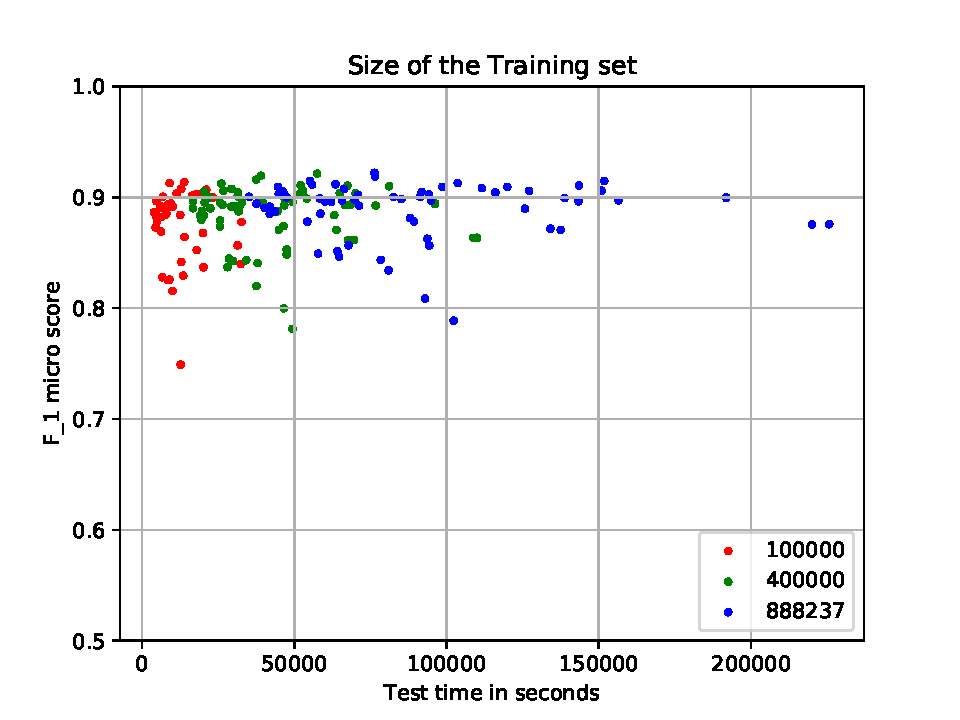
\includegraphics[width=1\linewidth]{fig/train_size__test_time__f1_micro}
%	\caption{Results for training set size -- test times}
%	\label{fig:train_size_test}
%\end{figure}

%\begin{figure}[htbp]
%	\centering
%	\subfigure[\label{fig:}]  {\centering
%		\includegraphics[width=.525\textwidth]{fig/}
%	}
%	\subfigure[\label{fig:}]  {\centering
%		\includegraphics[width=.525\textwidth]{fig/}
%	}
%	\caption{Evaluation results per parameter}
%	\label{fig:results2}
%\end{figure}


\subsubsection{Max\_iter}
%\begin{figure}[htbp]
%	\centering
%	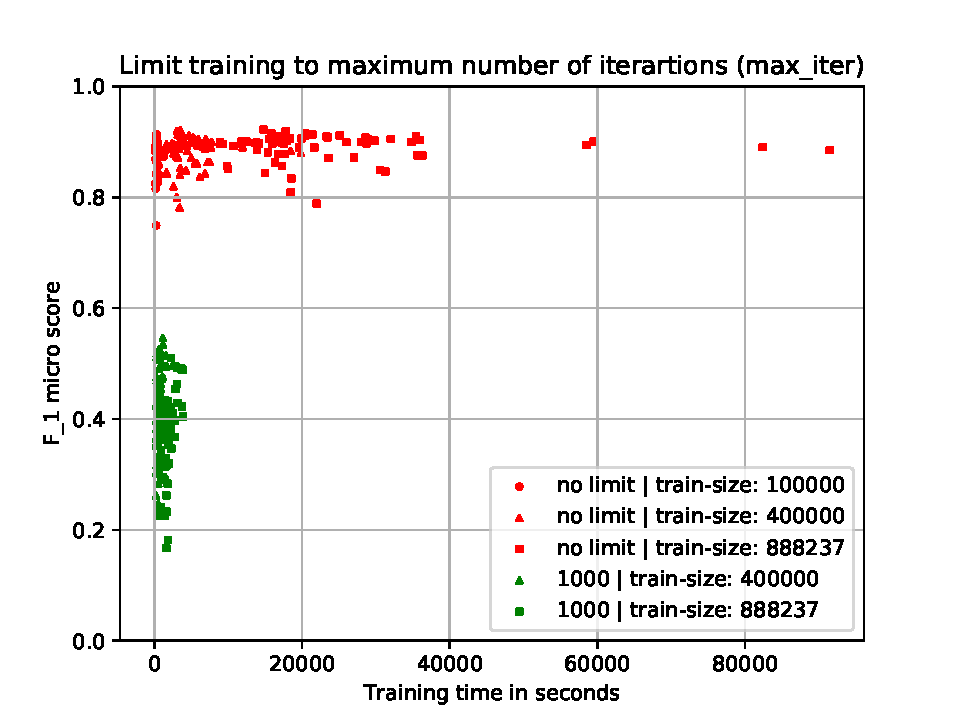
\includegraphics[width=1\linewidth]{fig/max_iter_train_size__train_time__f1_micro}
%	\caption{Results for parameter max\_iter}
%	\label{fig:max_iter}
%\end{figure}

As a first outcome it became obvious that limiting the maximum iterations for the solver resulted in bad scores, while however reducing the training times significantly (fig.~\ref{fig:max_iter}). When limiting to 1000 iterations the maximum training time was 3865 seconds compared to 34816 seconds without. But the F$_1$ scores were weak, especially when training on the full data set, with 0.600 at best on the 100k items data set. By hard limiting the solver, it was unable to find an optimal hyperplane. Therefore, the limiting was discarded and all other metrics were evaluated without limiting.

\subsubsection{Embedding dimensionality}
%\begin{figure}[htbp]
%	\centering
%	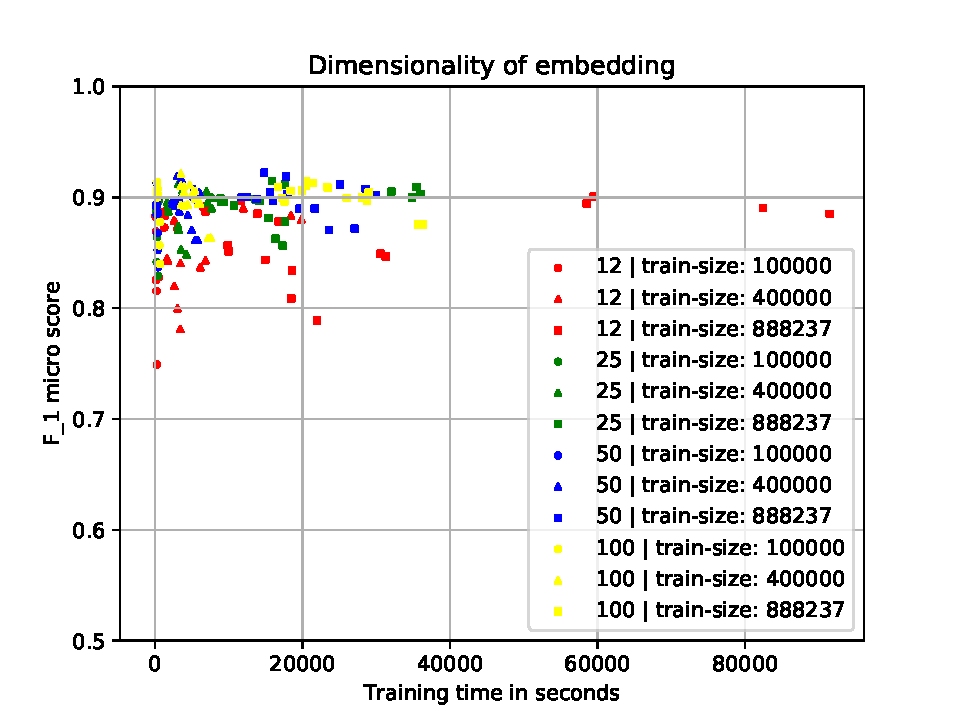
\includegraphics[width=1\linewidth]{fig/embedding_size_train_size__train_time__f1_micro}
%	\caption{Results for embedding size}
%	\label{fig:embedding_size}
%\end{figure}


\begin{table}[htbp]
	\caption{min train/test times, 400k dataset}
	\label{tab:embedding_size}
	\centering
	\begin{tabular}{lrr}
	\toprule
	{} &  train time &     test time \\
	\textbf{embedding size} &             &               \\
	\midrule
	\textbf{12            } &   75 &   3917 \\
	\textbf{25            } &   97 &   4757 \\
	\textbf{50            } &  154 &   6891 \\
	\textbf{100           } &  258 &  11419 \\
	\bottomrule
	\end{tabular}
\end{table}

The size of the embedding space played a role, but not as dominant as expected (fig.~\ref{fig:embedding_size}). On the full data set a dimensionality of 12 led to reduced training times at the cost of accuracy. The variance and sensitivity to other parameters decreases with increased dimensionality. A dimensionality of 50 provided excellent results for score (0.919) but also training time. A size of 100 performed slightly worse (0.914) while taking longer for training and testing. Also a small size of 25 offered notably good results (0.912).

Durations are hard to compare without all test results available. With especially the longest training and test times missing it is best to review the minimum durations (table~\ref{tab:embedding_size}).


\subsubsection{Embedding model}
%\begin{figure}[htbp]
%	\centering
%	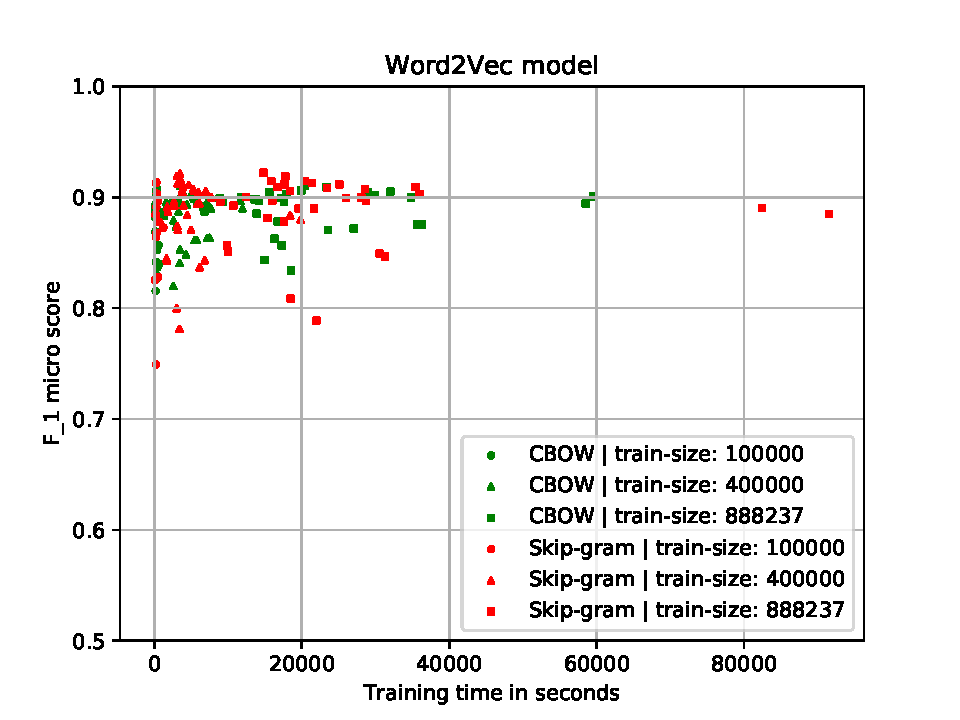
\includegraphics[width=1\linewidth]{fig/embedding_model_train_size__train_time__f1_micro}
%	\caption{Results for embedding model}
%	\label{fig:embedding_model}
%\end{figure}


\begin{table}[htbp]
	\caption{model -- max scores}
	\label{tab:embedding_model}
	\centering
	\begin{tabular}{lrrr}
	\toprule
		{} &  f1 micro &  f1 macro &  f1 weighted \\
		\textbf{model} &           &           & \\
		\midrule
		\textbf{sg    } &  0.919 &  0.835 &     0.910 \\
		\textbf{cb    } &  0.910 &  0.839 &     0.904 \\
		\bottomrule
	\end{tabular}
\end{table}

CBOW and Skip-gram are variants of word2vec model where -- in short -- the first is predicting a word based on a given context and the latter is predicting a context on a given word. The Skip-gram model is somewhat more advanced, but not always outperforming the CBOW model. In this challenge both models are very close to each other (fig.~\ref{fig:embedding_model}). While the Skip-gram model has slightly better maximum ratings for the F$_1$ micro and F$_1$ weighted scores (0.919 vs. 0.911 and 0.911 vs. 0.905), CBOW has a slightly higher max on F$_1$ macro and on mean scores over all models (table~\ref{tab:embedding_model}). Skip-gram seems to increase training times on bigger data sets. For smaller corpora we would recommend using Skip-gram, with bigger corpora CBOW.

\subsubsection{Case sensitivity}
%\begin{figure}[htbp]
%	\centering
%	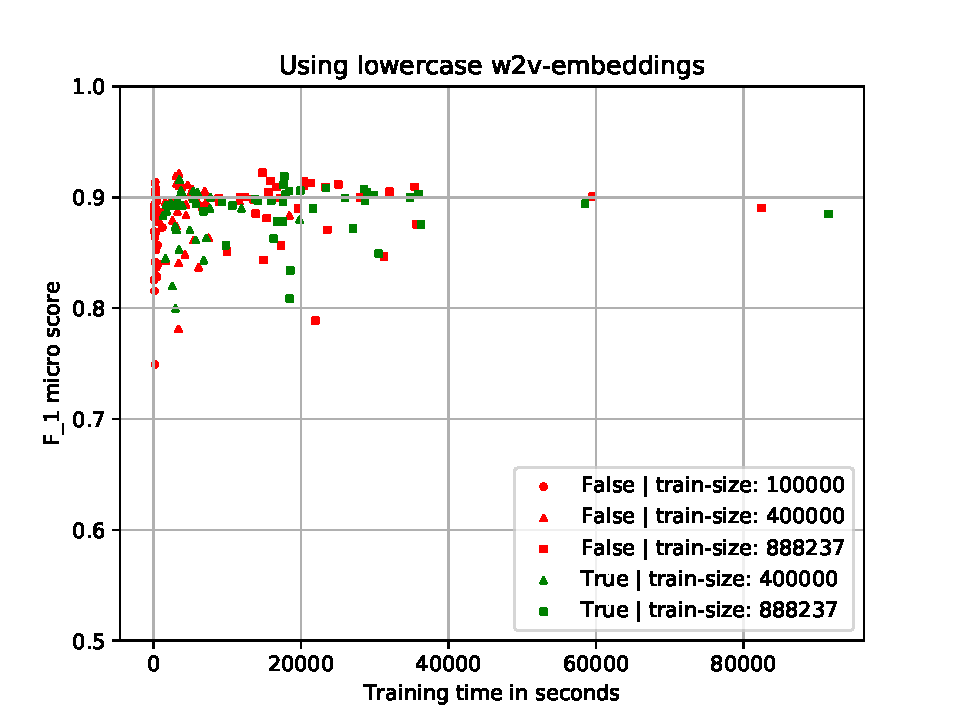
\includegraphics[width=1\linewidth]{fig/lowercase_train_size__train_time__f1_micro}
%	\caption{Results for case sensitivity}
%	\label{fig:lowercase}
%\end{figure}


\begin{table}[htbp]
	\caption{case sensitivity -- max scores}
	\label{tab:lowercase}
	\centering
	\begin{tabular}{lrrr}
	\toprule
		{} &  f1 micro &  f1 macro &  f1 weighted \\
		\textbf{lowercase} &           &           & \\
		\midrule
		\textbf{False} &  0.919 &  0.839 &     0.911 \\
		\textbf{True} &  0.916 &  0.836 &     0.908 \\
		\bottomrule
	\end{tabular}
\end{table}

Lowercase-only tokens reduce the score slightly while increasing the training times (fig.~\ref{fig:lowercase}, table~\ref{tab:lowercase}). Therefore, case-sensitive tokens are preferable. On additional tests with a 100k items data set we discarded lowercased inputs.

\subsubsection{C-parameter}
%\begin{figure}[htbp]
%	\centering
%	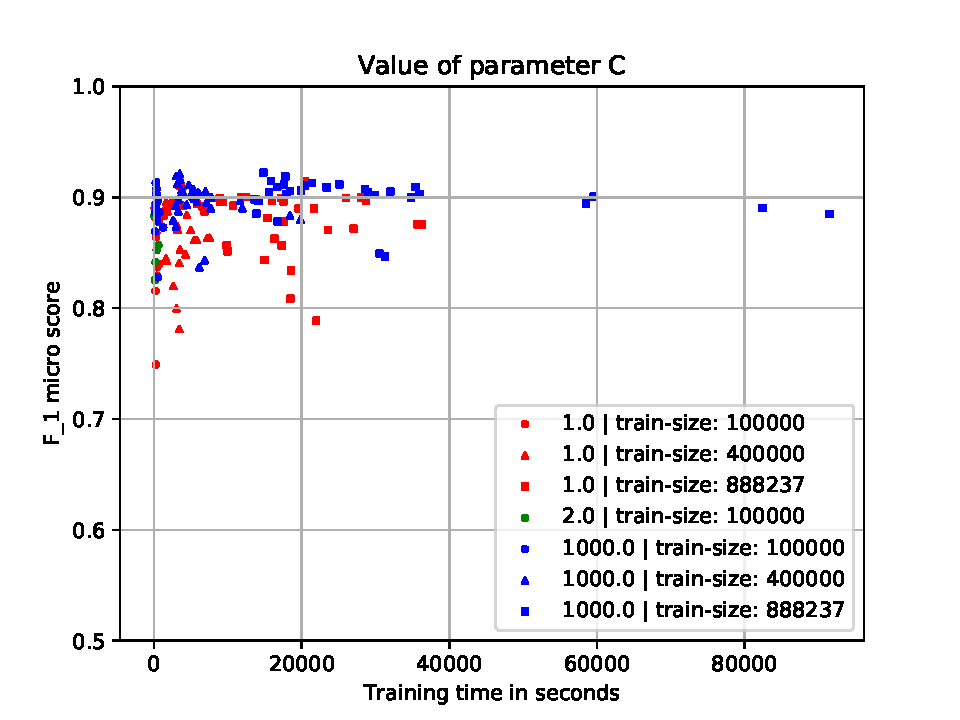
\includegraphics[width=1\linewidth]{fig/C_train_size__train_time__f1_micro}
%	\caption{Results for parameter C}
%	\label{fig:C}
%\end{figure}


\begin{table}[htbp]
	\caption{C -- max scores}
	\label{tab:C}
	\centering
	\begin{tabular}{lrrr}
	\toprule
		{} &  f1 micro &  f1 macro &  f1 weighted \\
		\textbf{C} &           &           & \\
		\midrule
		\textbf{1000.0} & 0.919   & 0.839  &    0.911  \\
		\textbf{2.0}    & 0.907   & 0.815  &    0.898  \\
		\textbf{1.0}    & 0.903   & 0.818  &    0.893  \\
		\bottomrule
	\end{tabular}
\end{table}

An unusually high value of 1000.0 for the soft-margin parameter C could indeed outperform the default of 1.0 (0.919 vs. 0.903, table~\ref{tab:C}), again at the expense of training time, especially for large corpora. Training times can be up to 2-5 times higher (fig.~\ref{fig:C}). Test times are roughly the same. Still for smaller corpora a high C setting is recommended.
We've have also performed some test on the 100k data set with a setting of 2.0, showing a very slight performance increase compared to 1.0 and roughly the same training/test durations.

\subsubsection{Scaling}
%\begin{figure}[htbp]
%	\centering
%	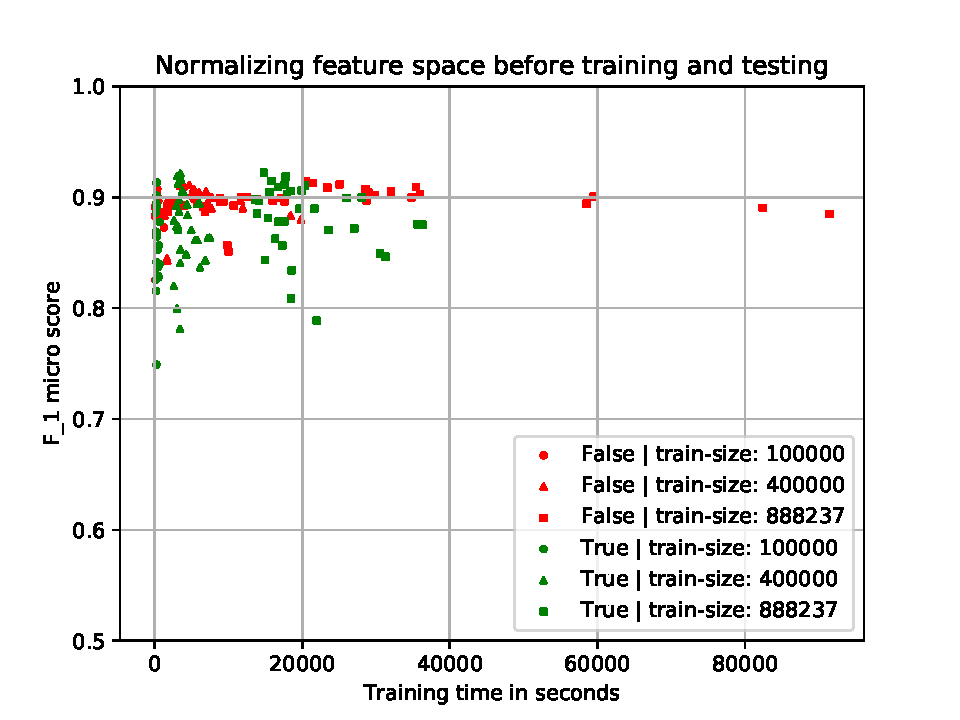
\includegraphics[width=1\linewidth]{fig/scale_train_size__train_time__f1_micro}
%	\caption{Results for scaling}
%	\label{fig:scale}
%\end{figure}


\begin{table}[htbp]
	\caption{Scaling -- max scores}
	\label{tab:scale_max}
	\centering
	\begin{tabular}{lrrr}
	\toprule
		{} &  f1 micro &  f1 macro &  f1 weighted \\
		\textbf{Scaling} &           &           & \\
		\midrule
		\textbf{True } & 0.919   & 0.829  &    0.911  \\
		\textbf{False} & 0.911   & 0.839  &    0.905  \\
		\bottomrule
	\end{tabular}
\end{table}


\begin{table}[htbp]
	\caption{Scaling -- mean scores}
	\label{tab:scale_mean}
	\centering
	\begin{tabular}{lrrr}
	\toprule
		{} &  f1 micro &  f1 macro &  f1 weighted \\
		\textbf{Scaling} &           &           & \\
		\midrule
		\textbf{False} &  0.891 &  0.809 &     0.883 \\
		\textbf{True } &  0.859 &  0.757 &     0.847 \\
		\bottomrule
	\end{tabular}
\end{table}


Normalizing word vectors prior to an SVM has some interesting effects. While it greatly reduces the variance on the time axis it also greatly increases the variance on the score axis (fig.~\ref{fig:scale}). The top scores come from models with scaled input vectors (table~\ref{tab:scale_max}), but the mean of all models lies below that of the unscaled data (0.859 vs. 0.891, table~\ref{tab:scale_mean}). Normalizing works well with high C values and should be used only in this combination.



\subsubsection{Training set size}
%\begin{figure}[htbp]
%	\centering
%	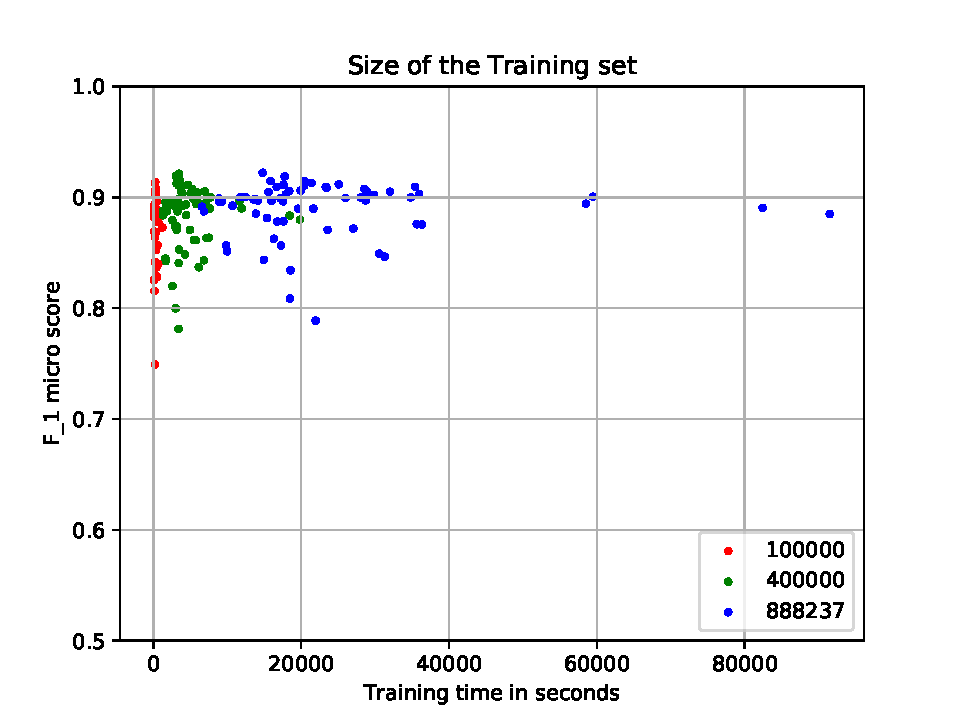
\includegraphics[width=1\linewidth]{fig/train_size__train_time__f1_micro}
%	\caption{Results for training set size}
%	\label{fig:train_size}
%\end{figure}
%
%
%\begin{figure}[htbp]
%	\centering
%	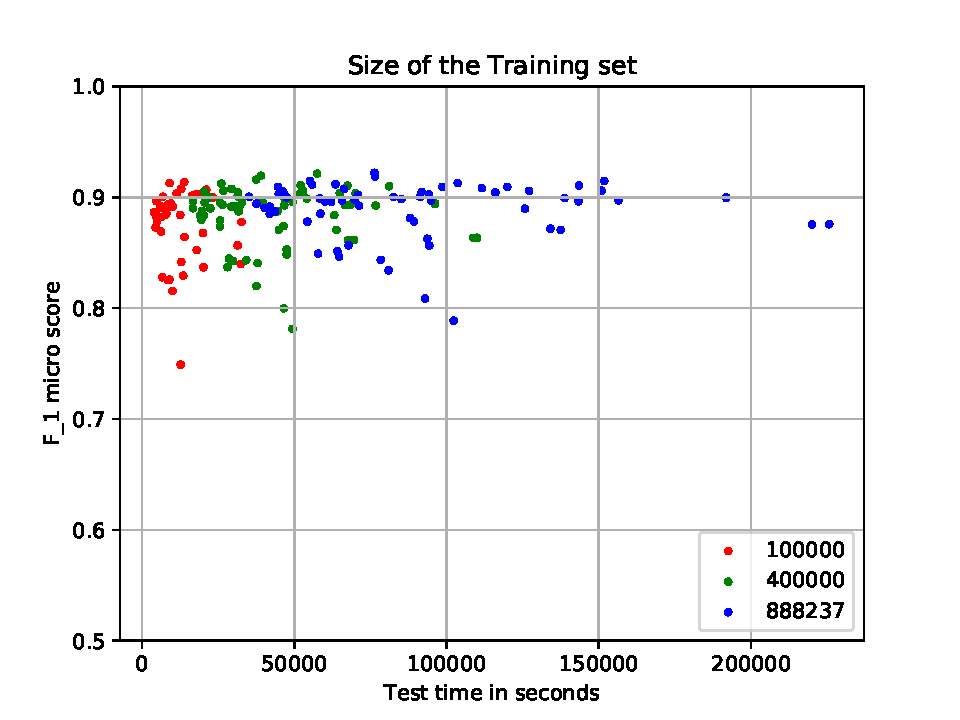
\includegraphics[width=1\linewidth]{fig/train_size__test_time__f1_micro}
%	\caption{Results for training set size -- test times}
%	\label{fig:train_size_test}
%\end{figure}


\begin{table}[htbp]
	\caption{Training data set size -- max scores}
	\label{tab:train_size}
	\centering
	\begin{tabular}{lrrr}
	\toprule
		{} &  f1 micro &  f1 macro &  f1 weighted \\
		\textbf{trainset} &           &           & \\
		\midrule
		\textbf{400k    } &  0.919 &  0.835 &     0.910 \\
		\textbf{100k    } &  0.913 &  0.825 &     0.905 \\
		\textbf{888k    } &  0.910 &  0.839 &     0.904 \\
		\bottomrule
	\end{tabular}
\end{table}

Our tests revealed, that very good scores can already be achieved with a comparatively small training data set (fig.~\ref{fig:train_size}, table~\ref{tab:train_size}). There is no benefit from increasing the data set. On the contrary: increasing the data set puts an exponential factor on training times, but increases also prediction times (fig.~\ref{fig:train_size_test}). This is presumably due to the rbf kernel which may get more complex with an increased amount of data. Finding an optimal hyperplane becomes exponentially harder with many data points. We would therefore recommend to use not more than half of the TIGER corpus for training.



\section{Conclusion and Future Work}
In this paper we propose an SVM based POS-tagger trained on the TIGER corpus using word embeddings as input data. The model is based only on the token itself without context of surrounding words. A maximum F$_1$ micro score of 0.919 when tested on the HDT corpus could be reached. For comparison: an NLTK POS-tagger trained on the same data set returns an F$_1$ micro score of only 0.873.

As an optimal parameter-set when working with scikit-learn's SVC class and rbf-kernel we recommend:
\begin{itemize*}
	\item embedding dimensionality: 50
	\item w2v-model: Skip-gram
	\item keep case sensitivity
	\item normalize vectors to [0,1]
	\item C: 1000.0
	\item training set: 400k tokens
\end{itemize*}

With very little decrease in accuracy (0.914) we can greatly speed-up the process by using only 100k tokens and an embedding size of 100.

If training on the entire corpus and still adequate training times are required we would recommend (for a score of 0.900):
\begin{itemize*}
	\item embedding dimensionality: 25
	\item w2v-model: CBOW
	\item keep case sensitivity
	\item no normalization
	\item C: 1.0
	\item training set: full
\end{itemize*}

The system is currently proof of concept. It demonstrates how well word embeddings retain syntactic and semantic information. It would be interesting to see if additional context tokens would improve the prediction score.

A linear kernel may be beneficial to speed up the process, probably in combination with an enlarged vector space. Training and test times are currently too slow. After all, an SVM is probably not be the best classifier for this sort of problem and will be even slower on larger tagsets. A neural network may be sensible alternative.


% include your own bib file like this:
%\bibliographystyle{acl}
%\bibliography{acl2017}
\bibliography{pos}
\bibliographystyle{acl_natbib}

\end{document}